

    \begin{figure}[htbp]
        \centering
        \begin{subfigure}[b]{0.48\textwidth}
            \centering
            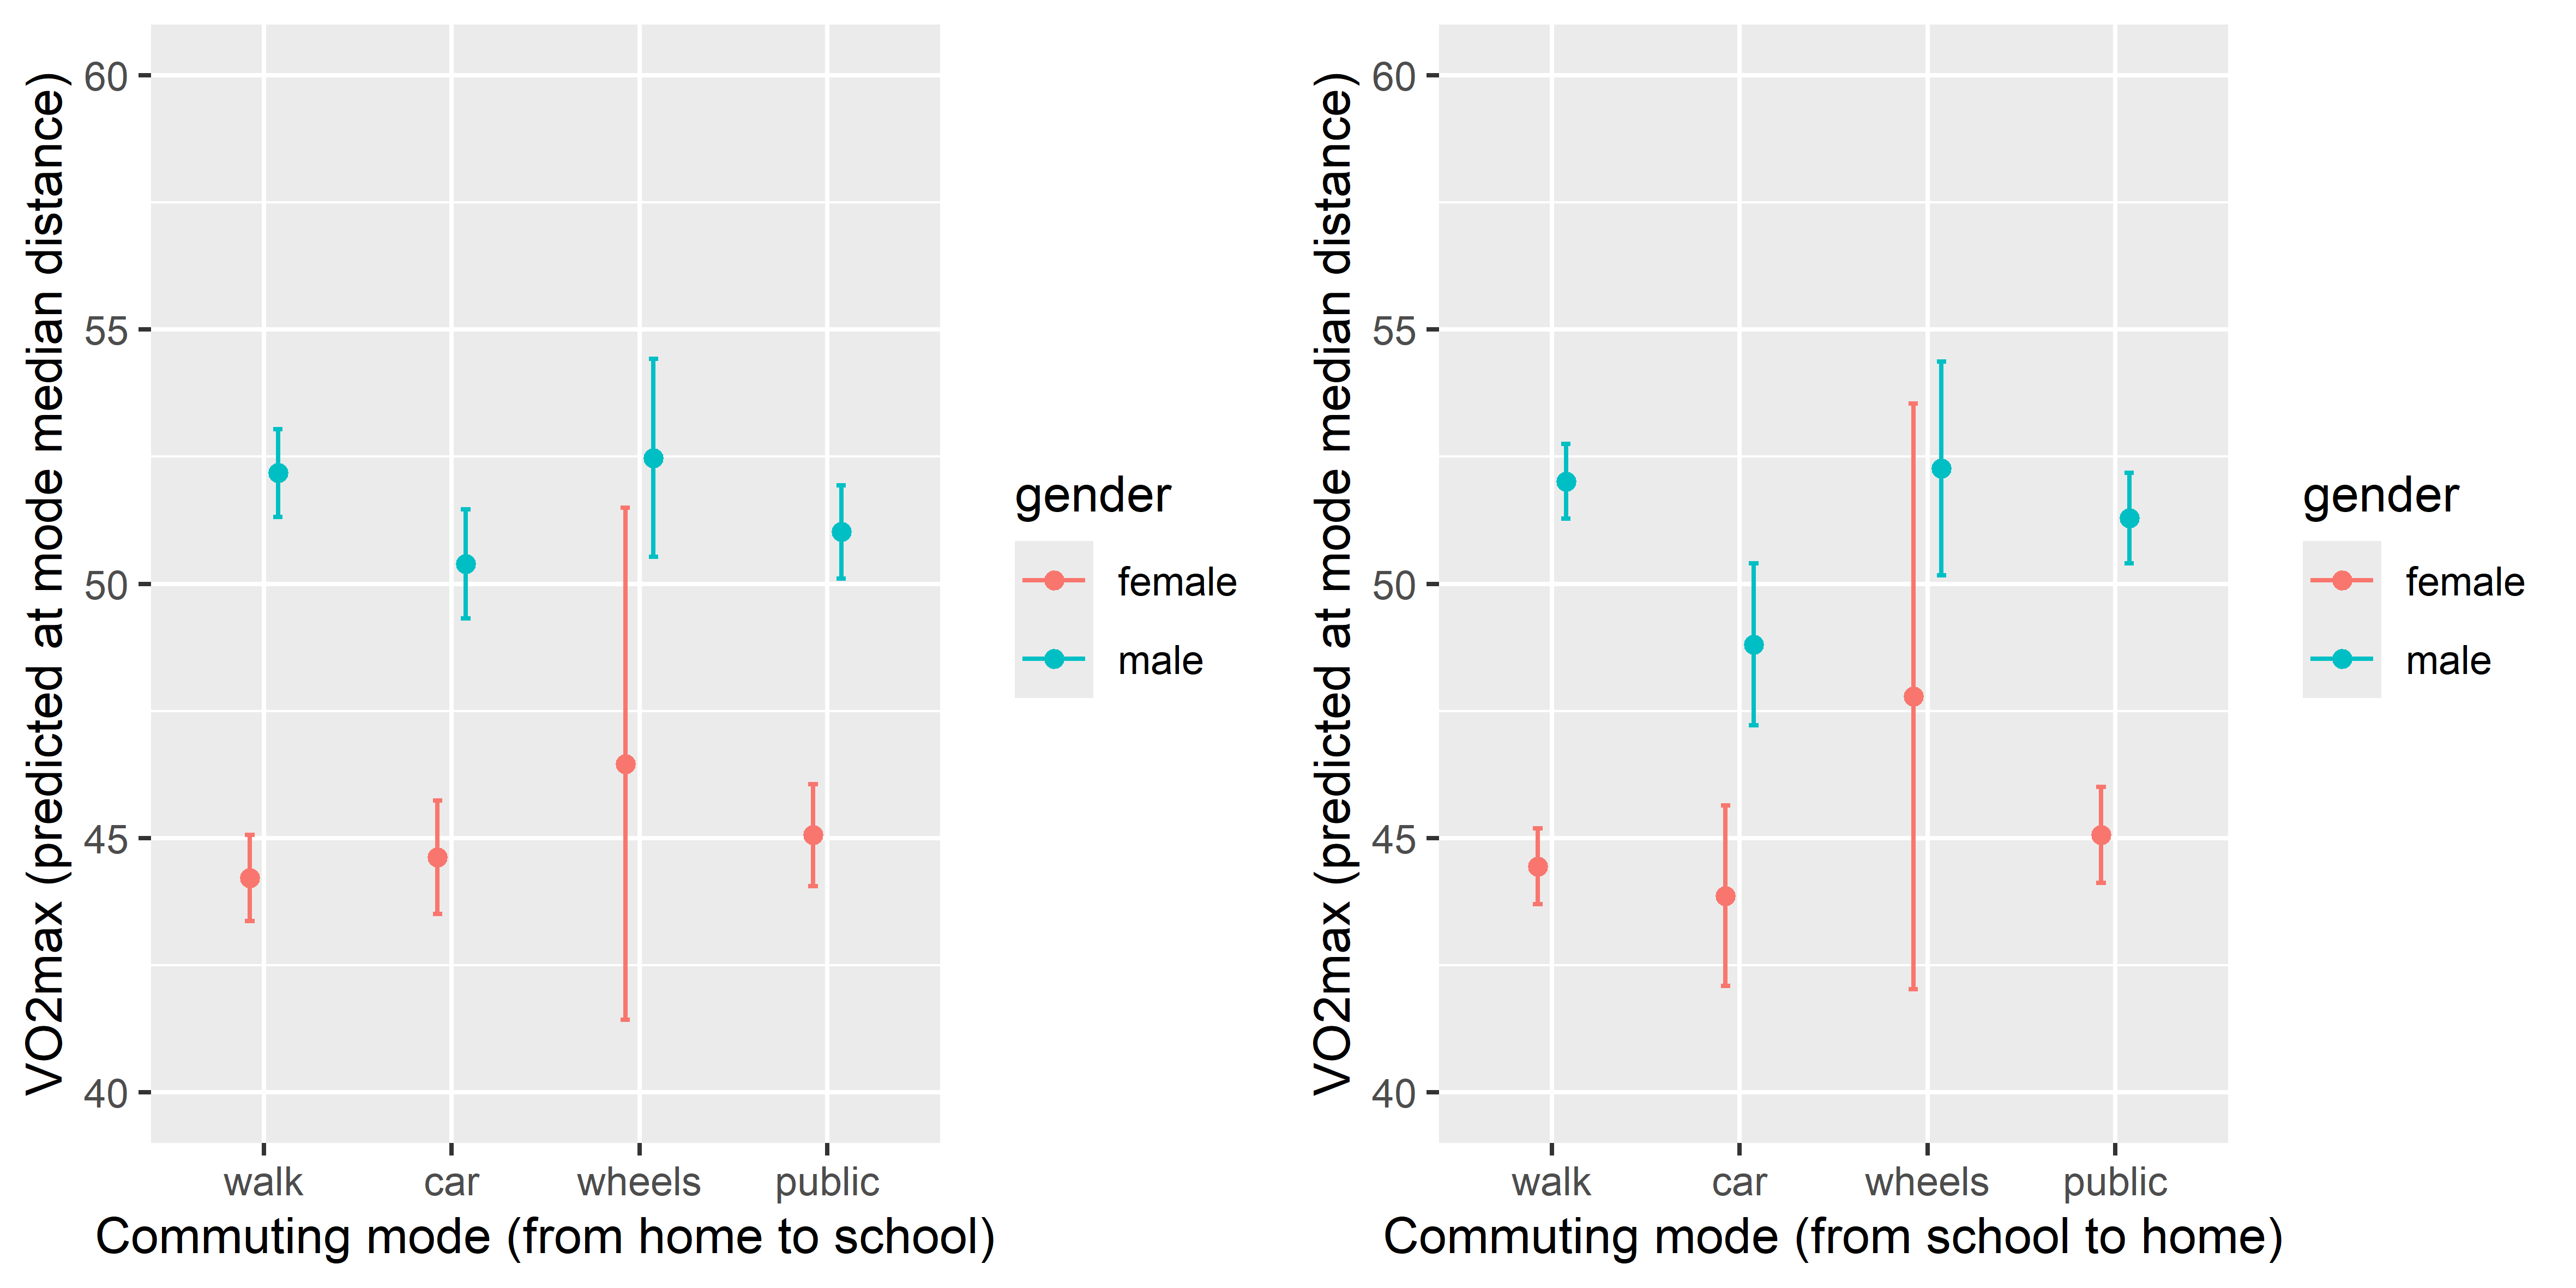
\includegraphics[width=\textwidth]{figs/r_orig_plot.png}
            \caption{Original Plot}
            \label{fig:r_orig_plot}
        \end{subfigure}
        \hspace{0.0\textwidth}
        \begin{subfigure}[b]{0.48\textwidth}
            \centering
            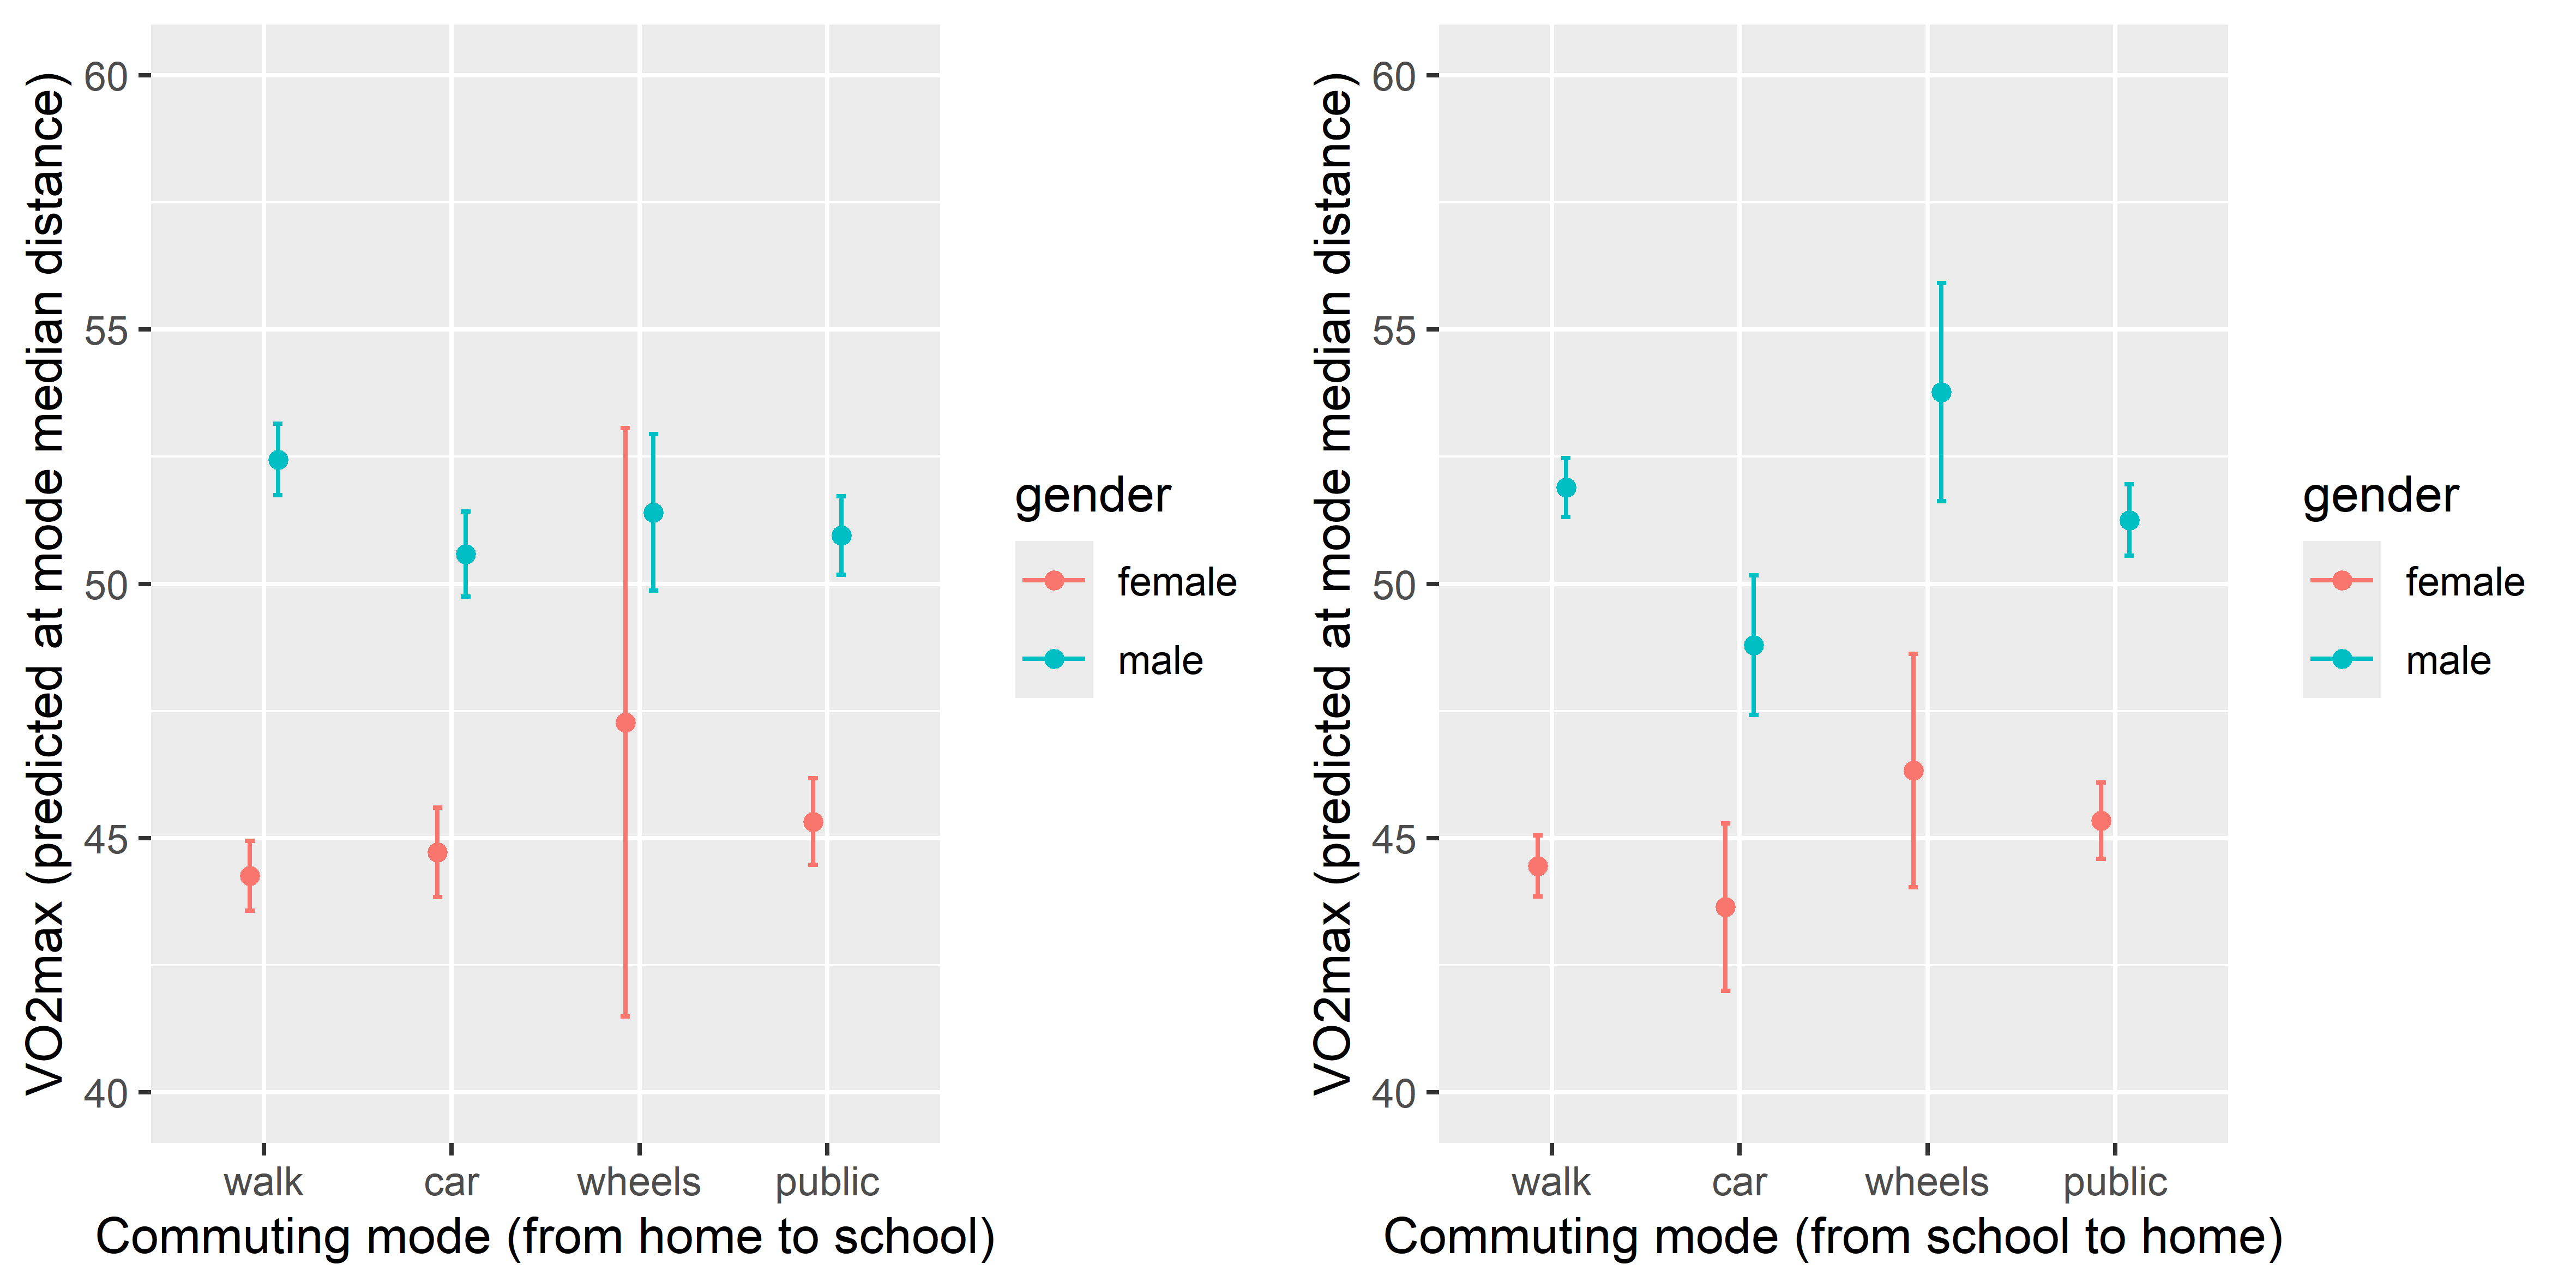
\includegraphics[width=\textwidth]{figs/r_arx_plot.png}
            \caption{ARX Plot}
            \label{fig:r_arx_plot}
        \end{subfigure}
        \vfill
        \begin{subfigure}[b]{0.48\textwidth}
            \centering
            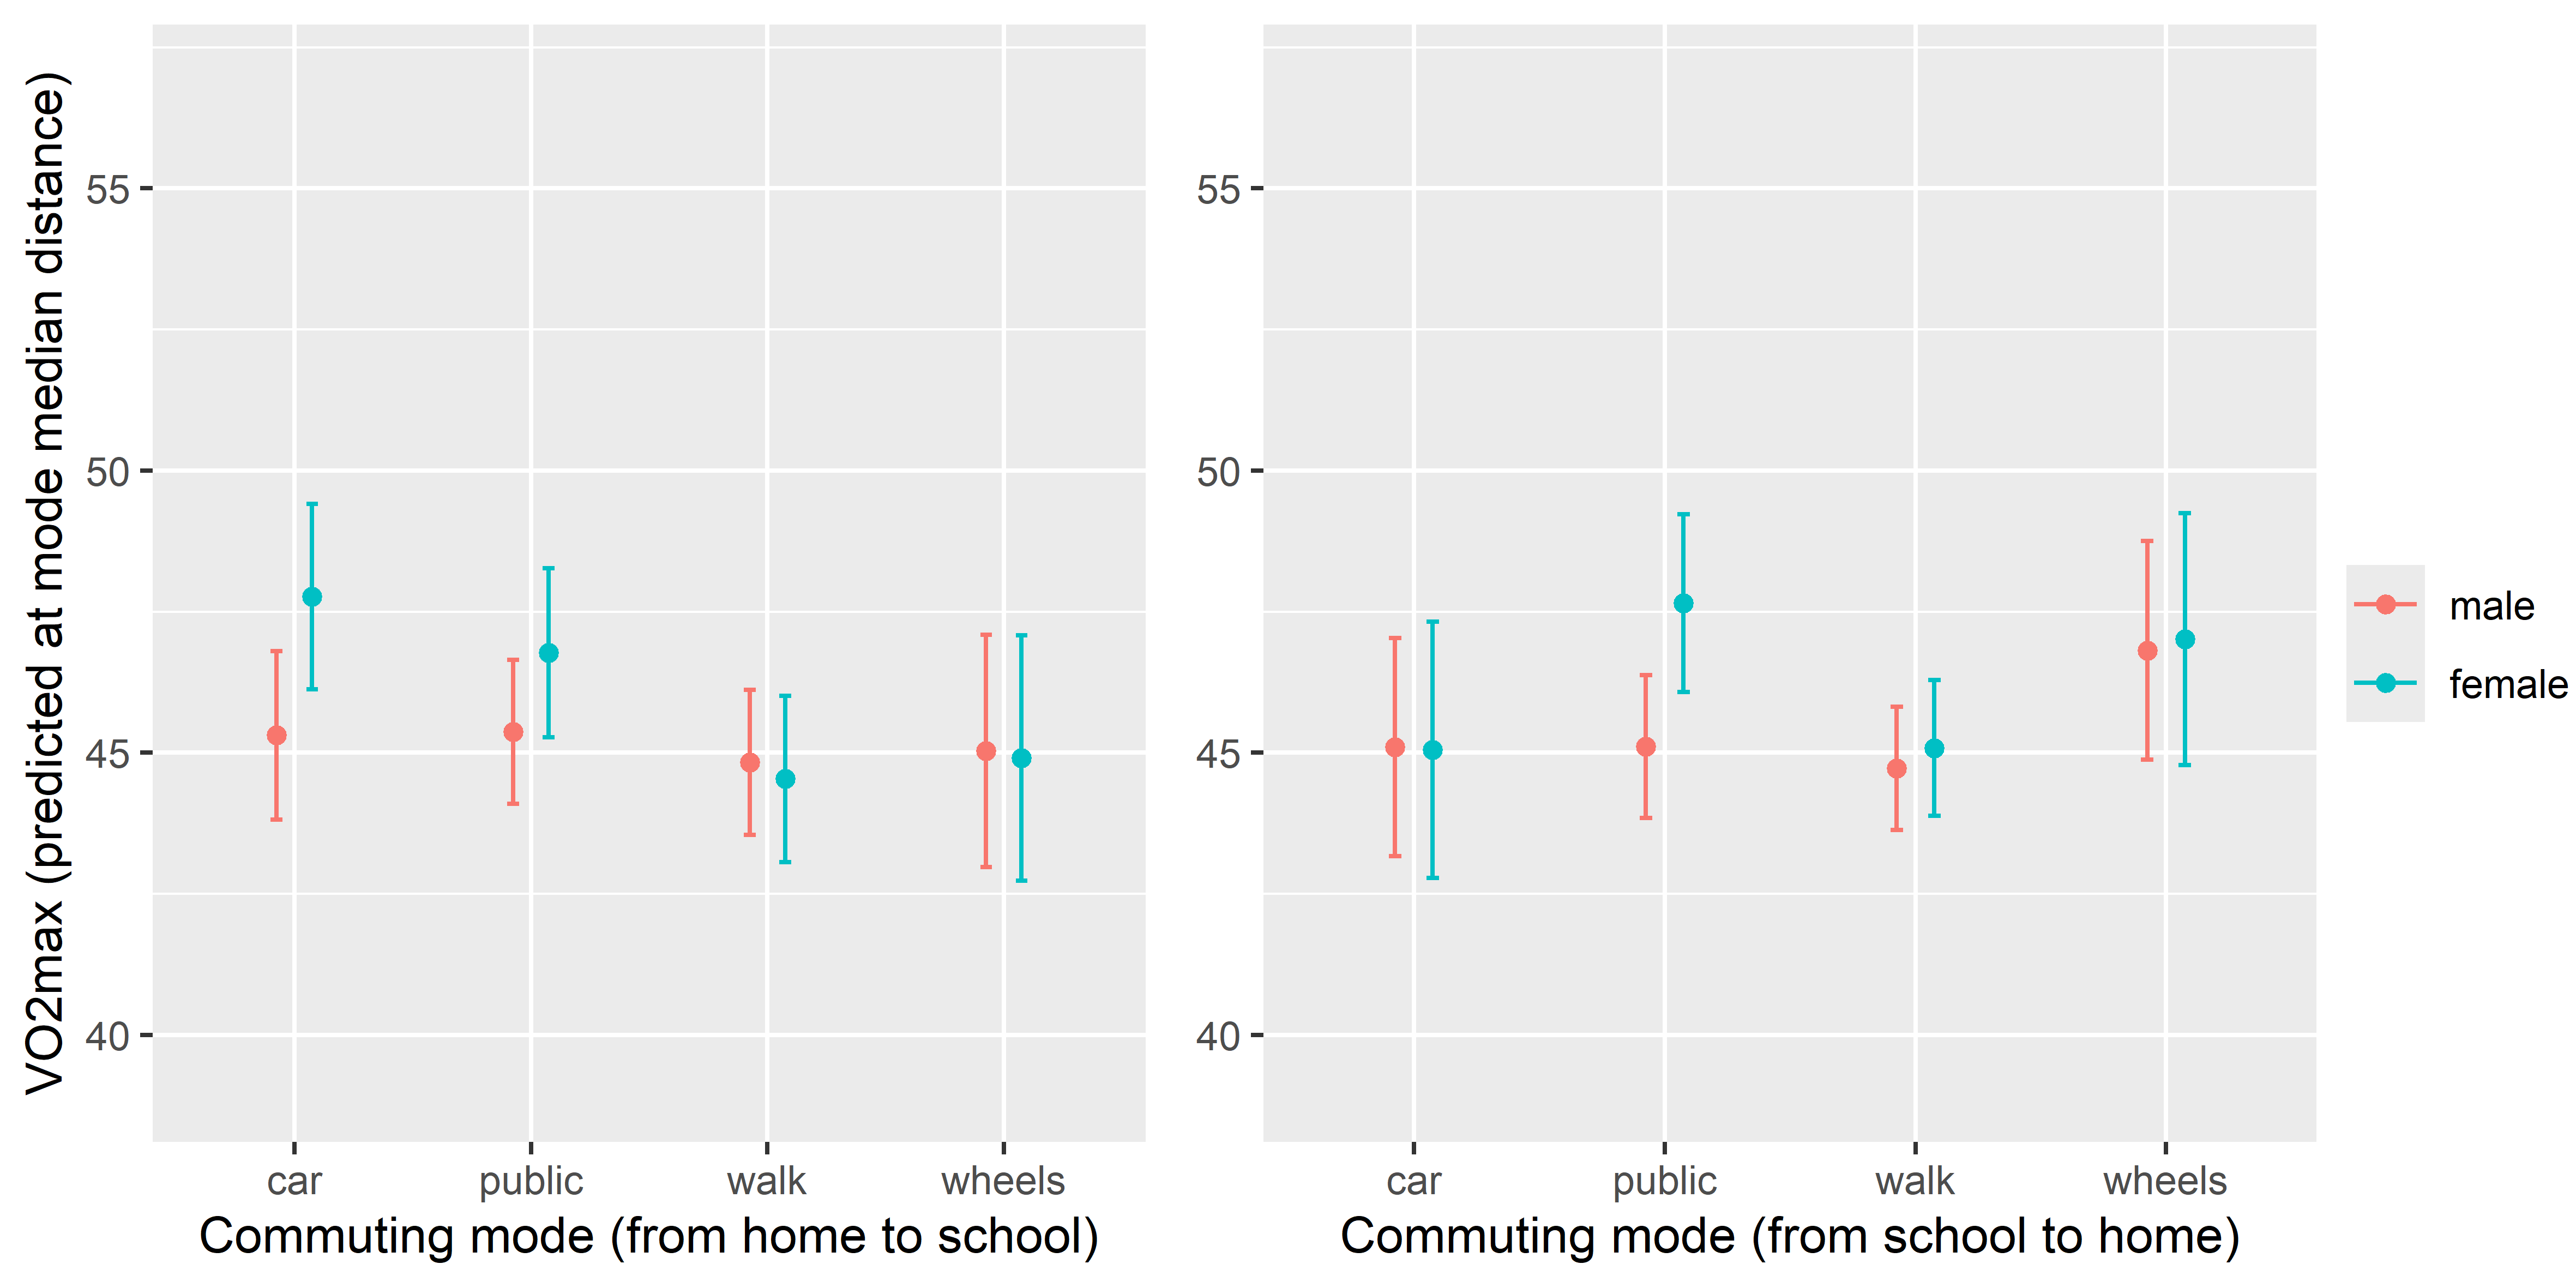
\includegraphics[width=\textwidth]{figs/r_sdv_plot.png}
            \caption{SDV Plot}
            \label{fig:r_sdv_plot}
        \end{subfigure}
        \hspace{0.0\textwidth}
        \begin{subfigure}[b]{0.48\textwidth}
            \centering
            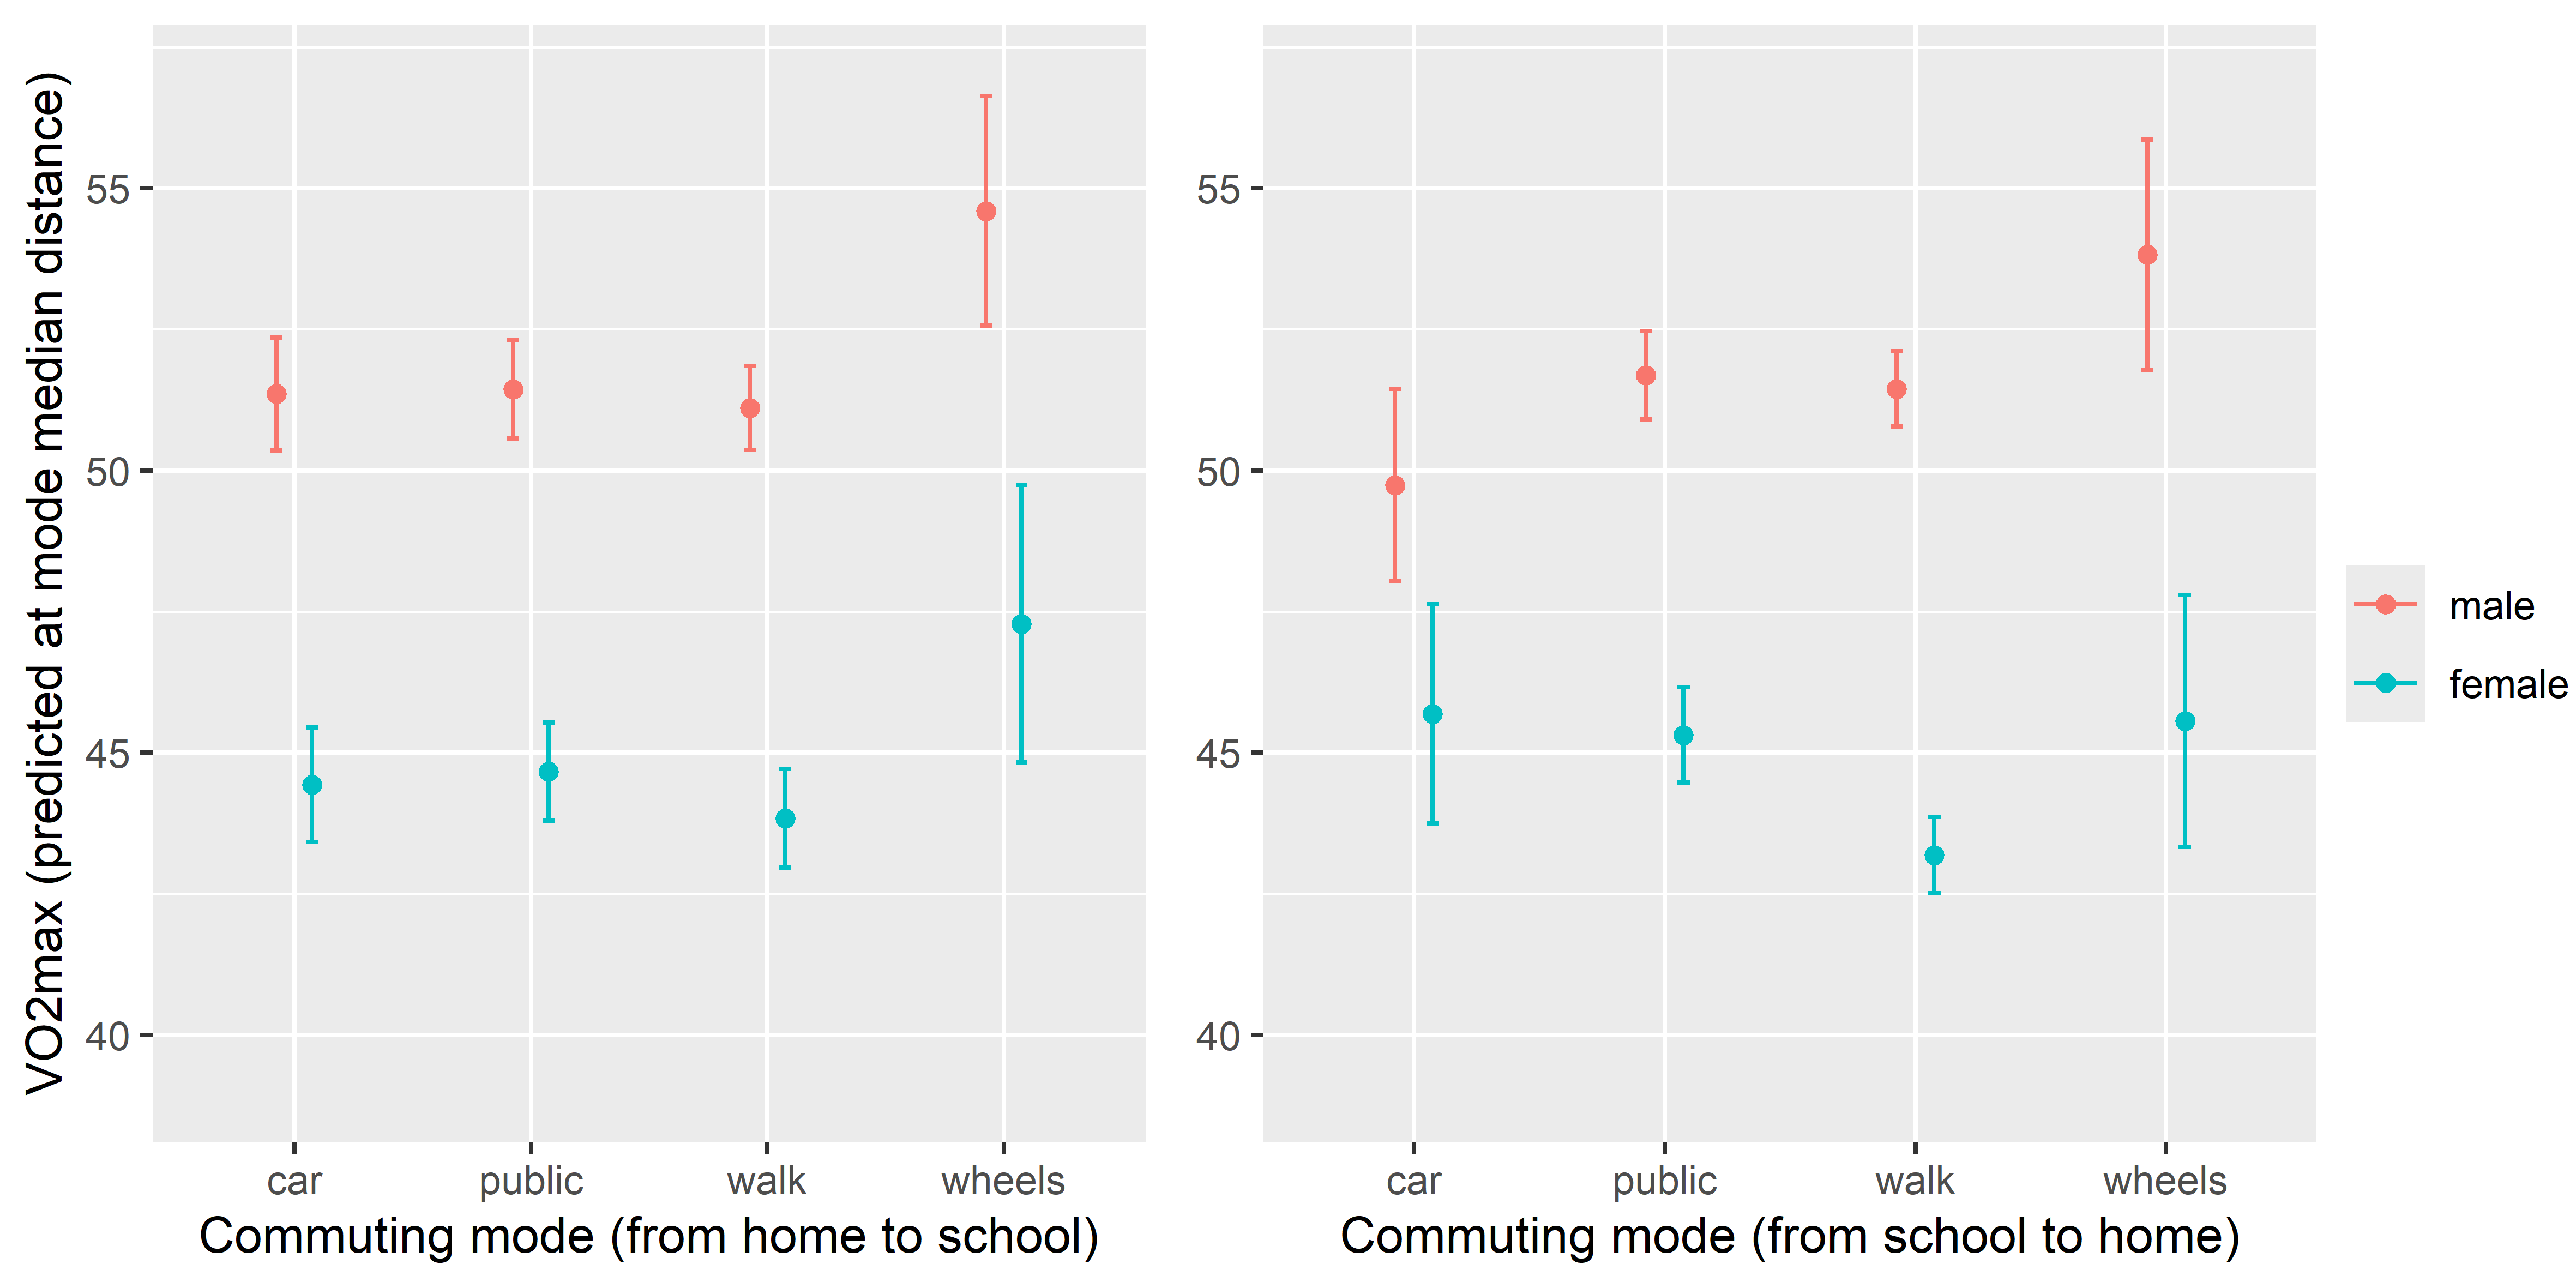
\includegraphics[width=\textwidth]{figs/r_sdx_plot.png}
            \caption{SynDiffix Plot}
            \label{fig:r_sdx_plot}
        \end{subfigure}

        \caption{Comparison of the VO2max data. Here we see that ARX matches very closely with the original data. SynDiffix is quite close for female, but for reasons I don't understand yet, does somewhat bad for the car commute for males. Otherwise, though SynDiffix is pretty good. SDV is again quite bad. What will be important is whether the correct conclusions can be drown from the data in spite of the error.
        }
        \label{fig:comparison_plots}
    \end{figure}

    